%\documentclass[windows,csize4]{BHCexam}
\documentclass[windows,csize4,answers]{BHCexam}

\usepackage{multicol} % 分栏
\pagestyle{fancy}
\fancyfoot[C]{\kaishu \small 第 \thepage 页 共 \pageref{lastpage} 页}
%\fancyhead[L]{\includegraphics[width=2cm]{qrcode.png}}
\title{因式分解 - 双十字相乘,主元法}
%\subtitle{数学文科试卷}
%\notice{满分150分, 120分钟完成, \\	允许使用计算器,答案一律写在答题纸上.}
%\author{Gavin Chen}
%\date{\today}
\usepackage{enumerate} % 编号


\begin{document}

\maketitle

\begin{groups}
    \group{双十字相乘概念}{}
    假设多项式
    \begin{equation}
        ax^2+bxy+cy^2+dx+ey+f \label{eq:factorization1}
    \end{equation}
    可以因式分解为
    \begin{equation}
        (mx+py+j)(nx+qy+k) \label{eq:factorization2}
    \end{equation}
    将\ref{eq:factorization2}展开可以得到
    \begin{equation}
        mnx^2+(mq+np)xy+pqy^2+(mk+nj)x+(pk+qj)y+kj \label{eq:factorization3}
    \end{equation}

    根据多项式相等的原理,由\ref{eq:factorization1}和\ref{eq:factorization3}可以得到:
    \begin{equation}
        \begin{cases}
            mn=a    \\
            mq+np=b \\
            pq=c    \\
            mk+nj=d \\
            pk+qj=e \\
            kj=f
        \end{cases}
        \label{eq:factorization4}
    \end{equation}
    所以可以得到双十字相乘
    \begin{figure}[htb]
        \centering
        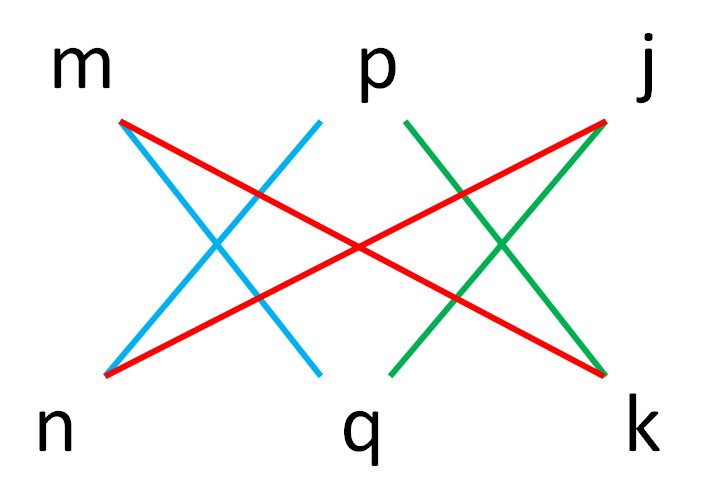
\includegraphics [scale=0.5,trim=0 0 0 0]{./image/U2_Factorization_1.png}
        \caption{双十字相乘示意图}
        \label{fig:factorization}
    \end{figure}
\end{groups}

\begin{groups}
    \group{双十字相乘例题}{}
    % 拆两个,凑一个
    \begin{questions}[]
        \begin{multicols}{2}
            \question[5]$(b+c)x^2-(b^2+c^2+3bc)x+bc(b+c)$
            \begin{solution}{0.5cm}
                \methodonly $[(b+c)x-bc][x-(b+c)]$
            \end{solution}

            \question[5]$x^2+2xy-3y^2+3x+y+2$
            \begin{solution}{0.5cm}
                \methodonly $(x+3y+2)(x-y+1)$
            \end{solution}
        \end{multicols}
        \vspace{3.5cm}

        \begin{multicols}{2}
            \question[5]$x^2-y^2+5x+3y+4$
            \begin{solution}{0.5cm}
                \methodonly $(x-y+4)(x+y+1)$
            \end{solution}

            \question[5]$x^2+3xy+2y^2+2x+2y+1$
            \begin{solution}{0.5cm}
                \methodonly $(x+y+1)(x+2y+1)$
            \end{solution}
        \end{multicols}

        \vspace{3.5cm}

        \begin{multicols}{2}
            \question[5]$x^2+2xy+y^2-3x-3y-40$
            \begin{solution}{0.5cm}
                \methodonly $(x+y-8)(x+y+5)$
            \end{solution}

            \question[5]$x^2-6xy+9y^2-5xz+15yz+6z^2$
            \begin{solution}{0.5cm}
                \methodonly $(x-3y-3z)(x-3y-2z)$
            \end{solution}
        \end{multicols}
        \vspace{3.5cm}

        \begin{multicols}{2}
            \question[5]$x^2-2xy-3y^2-2xz+10yz-3z^2$
            \begin{solution}{0.5cm}
                \methodonly $(x+y-3z)(x-3y+z)$
            \end{solution}

            \question[5]$6x^2-5xy-6y^2+2x+23y-20$
            \begin{solution}{0.5cm}
                \methodonly $(2x-3y+4)(3x+2y-5)$
            \end{solution}
        \end{multicols}
        \vspace{3.5cm}

        \begin{multicols}{2}
            \question[5]$2 x^2-x y+4 x z-6 y^2+13 y z-6 z^2$
            \begin{solution}{0.5cm}
                \methodonly $(2 x+3 y-2 z) (x-2 y+3 z)$
            \end{solution}

            \question[5]$6 x^2-x y+11 x z-12 y^2+26 y z-10 z^2$
            \begin{solution}{0.5cm}
                \methodonly $(3 x+4 y-2 z) (2 x-3 y+5 z)$
            \end{solution}
        \end{multicols}
        \vspace{3.5cm}

    \end{questions}
\end{groups}

\begin{groups}
    \group{主元法概念}{}
    \begin{itemize}
        \item 主要使用范围:含多个字母的复杂多项式(大部分情况下至少三个字母)
        \item 一般步骤:
              \begin{itemize}
                  \item 选某一个字母作为主元(当成未知数),其他当成常数
                  \item 按照这个字母降幂排列,并且合并同类项
                  \item 利用已有知识因式分解
                  \item 关键在于选主元,一个不行换一个
              \end{itemize}
    \end{itemize}
\end{groups}


\begin{groups}
    \group{主元法例题}{}
    \begin{questions}[]
        \question[5]$2x^3-x^2z-4x^2y+2xyz+2xy^2-y^2z$
        \begin{solution}{0.5cm}
            \methodonly 按照$x$为主元,得$2x^3-(z+4y)x^2+(2z+2y^2)x-y^2z$,貌似不行 \\
            此题可以按照$z$为主元处理 \\
            $-z(x^2-2xy+y^2)+2x(x^2-2xy+y^2)=(x-y)^2(2x-z)$
        \end{solution}
        \vspace{3.5cm}

        \question[5]$abc-ab-bc-ca+a+b+c-1$
        \begin{solution}{0.5cm}
            \methodonly
            \[
                \begin{aligned}
                     & \phantom{=}abc-ab-bc-ca+a+b+c-1 \\
                     & =a(bc-b-c+1)-(bc-b-c+1)         \\
                     & =(bc-b-c+1)(a-1)                \\
                     & =[b(c-1)-(c-1)](a-1)            \\
                     & =(c-1)(b-c)(a-1)
                \end{aligned}
            \]
        \end{solution}
        \vspace{3.5cm}

        \question[5]$a^2b^2c^2-a^2b^2-b^2c^2-c^2a^2+a^2+b^2+c^2-1$
        \begin{solution}{0.5cm}
            \methodonly $(a^2-1)(b^2-1)(c^2-1)=(a+1)(a-1)(b+1)(b-1)(c+1)(c-1)$
        \end{solution}
        \vspace{3.5cm}

        \question[5]$x^2-3xy-10y^2+x+9y-2$
        \begin{solution}{0.5cm}
            \methodonly 将$x$看作主元
            \[
                \begin{aligned}
                     & \phantom{=}x^2+(1-3y)x+(-10y^2+9y-2) \\
                     & =x^2+(1-3y)x+(-5y+2)(2y-1)           \\
                     & =(x-5y+2)(x+2y-1)
                \end{aligned}
            \]
            如果将$y$看作主元
            \[
                \begin{aligned}
                     & \phantom{=}-10y^2+(9-3x)y+(x^2+x-2) \\
                     & =-10y^2+(9-3x)y+(x+2)(x-1)          \\
                     & =(-5y+x+2)(2y+x-1)
                \end{aligned}
            \]
        \end{solution}
        \vspace{3.5cm}

        \question[5]$a^3b-ab^3+2a^2+2b^2+4$
        \begin{solution}{0.5cm}
            \methodonly 此题按照字母比较麻烦,可以把数字作为主元
            \[
                \begin{aligned}
                     & \phantom{=}a^3b-ab^3+2a^2+2b^2+4   \\
                     & =2^2+(a^2+b^2)\cdot 2+ab(a+b)(a-b) \\
                     & =[2+b(a+b)][2+a(a-b)]
                \end{aligned}
            \]
        \end{solution}
        \vspace{3.5cm}


    \end{questions}
\end{groups}


\label{lastpage}
\end{document}